\documentclass[12pt,a4paper]{article}
\usepackage[utf8]{inputenc}
\usepackage{graphicx}
\usepackage{hyperref}
\usepackage{listings}
\usepackage{xcolor}
\usepackage{geometry}
\usepackage{longtable}
\usepackage{enumitem}
\usepackage{tikz}
\usetikzlibrary{shapes,arrows,positioning,fit,calc}

\geometry{margin=2.5cm}

\title{Perangkat Lunak Manajemen Museum\\Dokumentasi Teknis}
\author{Tim Pengembang}
\date{\today}

\begin{document}

\maketitle
\tableofcontents
\newpage

\section{Pendahuluan}
Dokumen ini menyediakan dokumentasi komprehensif untuk Perangkat Lunak Manajemen Museum, termasuk arsitektur sistem, prosedur pemeliharaan, dan panduan penggunaan. Dokumentasi ini mencakup setiap file dalam proyek dan memberikan informasi rinci tentang tujuan, fungsionalitas, dan penggunaannya.

\section{Tinjauan Proyek}
Perangkat Lunak Manajemen Museum adalah aplikasi desktop berbasis Java yang dibuat menggunakan Swing untuk antarmuka pengguna. Sistem ini dirancang untuk mengelola operasi museum, termasuk otentikasi pengguna, fungsi administratif, dan fitur khusus pengguna.

\section{Arsitektur Sistem}

\subsection{Arsitektur Frontend}
Frontend dibangun menggunakan Java Swing, memberikan pengalaman aplikasi desktop yang kaya.

\begin{figure}[h]
\centering
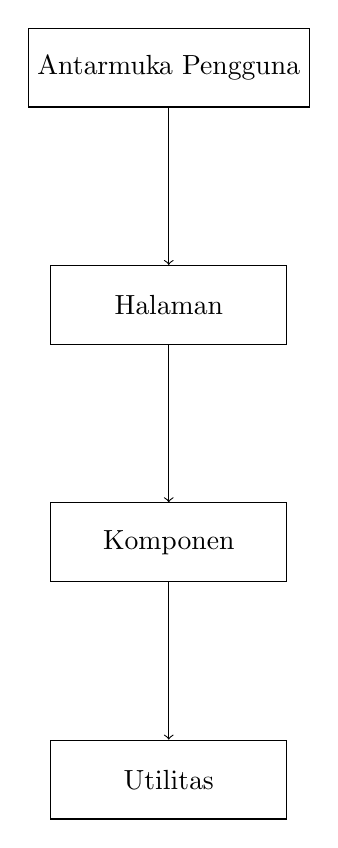
\begin{tikzpicture}[node distance=2cm]
    \node (ui) [rectangle, draw, minimum width=3cm, minimum height=1cm] {Antarmuka Pengguna};
    \node (pages) [rectangle, draw, below=of ui, minimum width=3cm, minimum height=1cm] {Halaman};
    \node (components) [rectangle, draw, below=of pages, minimum width=3cm, minimum height=1cm] {Komponen};
    \node (utils) [rectangle, draw, below=of components, minimum width=3cm, minimum height=1cm] {Utilitas};
    
    \draw [->] (ui) -- (pages);
    \draw [->] (pages) -- (components);
    \draw [->] (components) -- (utils);
\end{tikzpicture}
\caption{Lapisan Arsitektur Frontend}
\end{figure}

\subsubsection{Kerangka Kerja UI}
\begin{itemize}
    \item \textbf{Tumpukan Teknologi}
    \begin{itemize}
        \item Java Swing untuk komponen UI
        \item Komponen UI kustom di direktori \texttt{Components/}
        \item Arsitektur berbasis peristiwa (event-driven)
        \item Implementasi pola MVC
    \end{itemize}
    
    \item \textbf{Komponen Kunci}
    \begin{itemize}
        \item Kartu kustom untuk tampilan item
        \item Sistem navigasi
        \item Komponen formulir
        \item Widget tampilan data
    \end{itemize}
    
    \item \textbf{Organisasi UI}
    \begin{itemize}
        \item Antarmuka berbasis peran (Admin/Pengguna)
        \item Tata letak responsif
        \item Gaya yang konsisten
        \item Fitur aksesibilitas
    \end{itemize}
\end{itemize}

\subsubsection{Lapisan Antarmuka Pengguna}
\begin{itemize}
    \item \textbf{Lapisan Presentasi}
    \begin{itemize}
        \item Direktori \texttt{Pages/} berisi semua frame UI
        \item Direktori \texttt{Components/} untuk elemen UI yang dapat digunakan kembali
        \item Gaya dan tema kustom
        \item Penangan dan pendengar peristiwa (event handlers and listeners)
    \end{itemize}
    
    \item \textbf{Model Tampilan (View Models)}
    \begin{itemize}
        \item Implementasi pengikatan data (data binding)
        \item Manajemen status (state management)
        \item Mekanisme pembaruan UI
        \item Logika validasi
    \end{itemize}
\end{itemize}

\subsection{Arsitektur Middleware}
Lapisan middleware menangani logika bisnis, pemrosesan data, dan komunikasi antara frontend dan backend.

\begin{figure}[h]
\centering
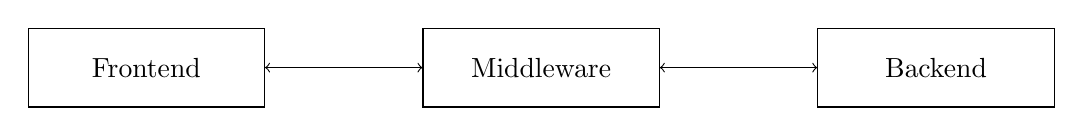
\begin{tikzpicture}[node distance=2cm]
    \node (frontend) [rectangle, draw, minimum width=3cm, minimum height=1cm] {Frontend};
    \node (middleware) [rectangle, draw, right=of frontend, minimum width=3cm, minimum height=1cm] {Middleware};
    \node (backend) [rectangle, draw, right=of middleware, minimum width=3cm, minimum height=1cm] {Backend};
    
    \draw [<->] (frontend) -- (middleware);
    \draw [<->] (middleware) -- (backend);
\end{tikzpicture}
\caption{Alur Komunikasi Middleware}
\end{figure}

\subsubsection{Lapisan Logika Bisnis}
\begin{itemize}
    \item \textbf{Komponen Inti}
    \begin{itemize}
        \item \texttt{Components/Utilities/} untuk logika bisnis
        \item Validasi dan pemrosesan data
        \item Implementasi aturan bisnis
        \item Manajemen status
    \end{itemize}
    
    \item \textbf{Lapisan Layanan (Service Layer)}
    \begin{itemize}
        \item Layanan otentikasi
        \item Layanan pemrosesan data
        \item Layanan penanganan gambar
        \item Layanan pencarian dan filter
    \end{itemize}
    
    \item \textbf{Lapisan Akses Data (Data Access Layer)}
    \begin{itemize}
        \item Manajemen koneksi basis data
        \item Eksekusi kueri
        \item Penanganan transaksi
        \item Pemetaan data
    \end{itemize}
\end{itemize}

\subsubsection{Lapisan Integrasi}
\begin{itemize}
    \item \textbf{Transformasi Data}
    \begin{itemize}
        \item Pemetaan objek-relasional
        \item Konversi format data
        \item Aturan validasi
        \item Penanganan kesalahan
    \end{itemize}
    
    \item \textbf{Komunikasi}
    \begin{itemize}
        \item Komunikasi frontend-backend
        \item Propagasi peristiwa
        \item Sinkronisasi status
        \item Propagasi kesalahan
    \end{itemize}
\end{itemize}

\subsection{Arsitektur Backend}
Backend dibangun di atas basis data MySQL dengan utilitas pemrosesan data kustom.

\begin{figure}[h]
\centering
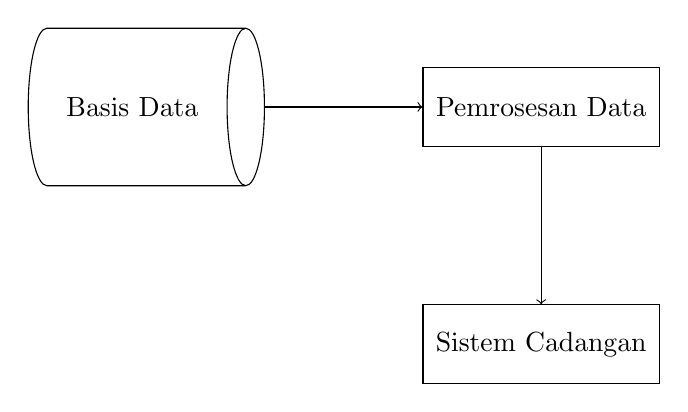
\begin{tikzpicture}[node distance=2cm]
    \node (db) [cylinder, draw, minimum width=2cm, minimum height=3cm] {Basis Data};
    \node (processing) [rectangle, draw, right=of db, minimum width=3cm, minimum height=1cm] {Pemrosesan Data};
    \node (backup) [rectangle, draw, below=of processing, minimum width=3cm, minimum height=1cm] {Sistem Cadangan};
    
    \draw [->] (db) -- (processing);
    \draw [->] (processing) -- (backup);
\end{tikzpicture}
\caption{Komponen Arsitektur Backend}
\end{figure}

\subsubsection{Lapisan Basis Data}
\begin{itemize}
    \item \textbf{Desain Basis Data}
    \begin{itemize}
        \item Skema basis data MySQL
        \item Hubungan antar tabel
        \item Optimalisasi indeks
        \item Manajemen batasan (constraint)
    \end{itemize}
    
    \item \textbf{Manajemen Data}
    \begin{itemize}
        \item Operasi CRUD
        \item Manajemen transaksi
        \item Pencadangan dan pemulihan
        \item Integritas data
    \end{itemize}
    
    \item \textbf{Optimalisasi Kueri}
    \begin{itemize}
        \item Kueri terindeks
        \item Prosedur tersimpan (stored procedures)
        \item Caching kueri
        \item Pemantauan kinerja
    \end{itemize}
\end{itemize}

\subsubsection{Pemrosesan Data}
\begin{itemize}
    \item \textbf{Alat Data}
    \begin{itemize}
        \item \texttt{get\_data.py} untuk pemrosesan data
        \item Skrip validasi data
        \item Utilitas impor/ekspor
        \item Alat transformasi data
    \end{itemize}
    
    \item \textbf{Sistem Cadangan}
    \begin{itemize}
        \item Pencadangan otomatis
        \item Pemulihan data
        \item Kontrol versi
        \item Manajemen arsip
    \end{itemize}
\end{itemize}

\subsubsection{Lapisan Keamanan}
\begin{itemize}
    \item \textbf{Otentikasi}
    \begin{itemize}
        \item Otentikasi pengguna
        \item Kontrol akses berbasis peran
        \item Manajemen sesi
        \item Keamanan kata sandi
    \end{itemize}
    
    \item \textbf{Perlindungan Data}
    \begin{itemize}
        \item Enkripsi data
        \item Komunikasi aman
        \item Pencatatan akses (logging)
        \item Pemantauan keamanan
    \end{itemize}
\end{itemize}

\section{Sistem Koneksi dan Alur Data}

\subsection{Arsitektur Koneksi Basis Data}
Aplikasi ini mengimplementasikan sistem koneksi basis data terpusat melalui kelas utilitas \texttt{DatabaseConnection}.

\begin{figure}[h]
\centering
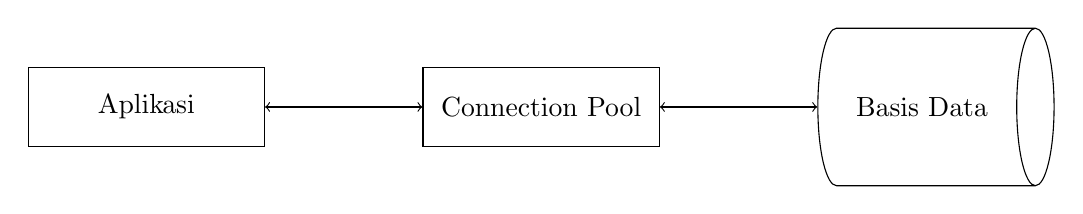
\begin{tikzpicture}[node distance=2cm]
    \node (app) [rectangle, draw, minimum width=3cm, minimum height=1cm] {Aplikasi};
    \node (pool) [rectangle, draw, right=of app, minimum width=3cm, minimum height=1cm] {Connection Pool};
    \node (db) [cylinder, draw, right=of pool, minimum width=2cm, minimum height=3cm] {Basis Data};
    
    \draw [<->] (app) -- (pool);
    \draw [<->] (pool) -- (db);
\end{tikzpicture}
\caption{Arsitektur Koneksi Basis Data}
\end{figure}

\subsection{Contoh Alur Data}

\subsubsection{Alur Tampilan Koleksi}
\begin{figure}[h]
\centering
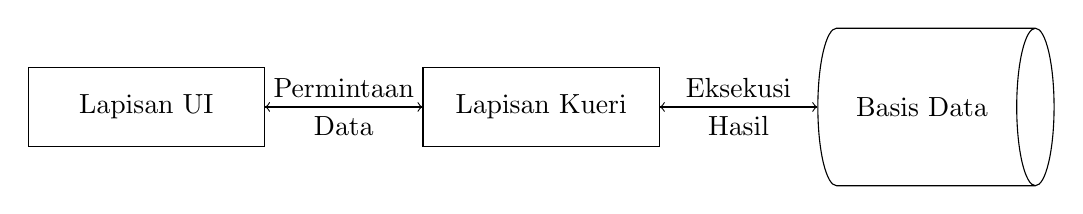
\begin{tikzpicture}[node distance=2cm]
    \node (ui) [rectangle, draw, minimum width=3cm, minimum height=1cm] {Lapisan UI};
    \node (query) [rectangle, draw, right=of ui, minimum width=3cm, minimum height=1cm] {Lapisan Kueri};
    \node (db) [cylinder, draw, right=of query, minimum width=2cm, minimum height=3cm] {Basis Data};
    
    \draw [->] (ui) -- node[above] {Permintaan} (query);
    \draw [->] (query) -- node[above] {Eksekusi} (db);
    \draw [->] (db) -- node[below] {Hasil} (query);
    \draw [->] (query) -- node[below] {Data} (ui);
\end{tikzpicture}
\caption{Alur Data Tampilan Koleksi}
\end{figure}

\begin{enumerate}
    \item \texttt{MuseumCollection.java} memulai permintaan data
    \item Memanggil \texttt{ItemQueries.getCollectionItems()}
    \item \texttt{DatabaseConnection} mengeksekusi kueri
    \item ResultSet dikembalikan ke \texttt{MuseumCollection}
    \item Data diproses oleh \texttt{ContainerPopulator}
    \item Ditampilkan melalui komponen \texttt{ItemCard}
\end{enumerate}

\subsubsection{Alur Manajemen Item}
\begin{enumerate}
    \item \texttt{AddItem.java} mengumpulkan data item
    \item Memvalidasi melalui \texttt{validateItemInput()}
    \item Memanggil \texttt{ItemQueries.insertItem()}
    \item \texttt{DatabaseConnection} mengeksekusi insert
    \item Transaksi di-commit
    \item UI diperbarui melalui \texttt{ContainerPopulator}
\end{enumerate}

\subsubsection{Implementasi Pencarian}
\begin{enumerate}
    \item \texttt{SearchBar.java} menangkap input pengguna
    \item Memicu \texttt{ItemQueries.searchItems()}
    \item \texttt{DatabaseConnection} mengeksekusi kueri pencarian
    \item Hasil diproses oleh \texttt{ContainerPopulator}
    \item Ditampilkan di tampilan \texttt{MuseumCollection}
\end{enumerate}

\subsection{Manajemen Koneksi}

\begin{figure}[h]
\centering
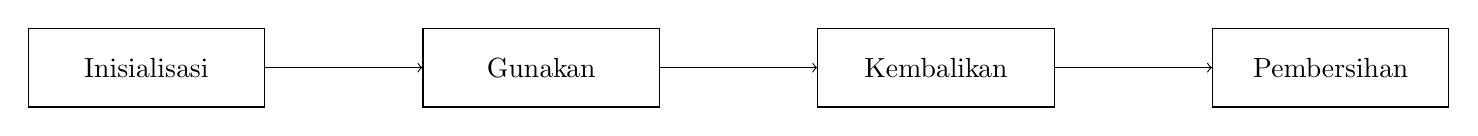
\begin{tikzpicture}[node distance=2cm]
    \node (init) [rectangle, draw, minimum width=3cm, minimum height=1cm] {Inisialisasi};
    \node (use) [rectangle, draw, right=of init, minimum width=3cm, minimum height=1cm] {Gunakan};
    \node (return) [rectangle, draw, right=of use, minimum width=3cm, minimum height=1cm] {Kembalikan};
    \node (clean) [rectangle, draw, right=of return, minimum width=3cm, minimum height=1cm] {Pembersihan};
    
    \draw [->] (init) -- (use);
    \draw [->] (use) -- (return);
    \draw [->] (return) -- (clean);
\end{tikzpicture}
\caption{Siklus Hidup Koneksi}
\end{figure}

\subsubsection{Penanganan Sumber Daya}
\begin{itemize}
    \item \textbf{Siklus Hidup Koneksi}
    \begin{itemize}
        \item Koneksi diperoleh dari pool
        \item Digunakan untuk eksekusi kueri
        \item Dikembalikan ke pool setelah digunakan
        \item Pembersihan otomatis saat aplikasi keluar
    \end{itemize}
    
    \item \textbf{Pemulihan Kesalahan}
    \begin{itemize}
        \item Penanganan waktu habis koneksi (timeout)
        \item Upaya koneksi ulang otomatis
        \item Pencatatan dan pelaporan kesalahan
        \item Sistem notifikasi pengguna
    \end{itemize}
\end{itemize}

\subsubsection{Optimalisasi Kinerja}
\begin{itemize}
    \item \textbf{Connection Pooling}
    \begin{itemize}
        \item Manajemen ukuran pool tetap
        \item Penggunaan kembali koneksi
        \item Pembersihan koneksi idle
        \item Pemantauan pool
    \end{itemize}
    
    \item \textbf{Optimalisasi Kueri}
    \begin{itemize}
        \item Caching prepared statement
        \item Dukungan operasi batch
        \item Streaming ResultSet
        \item Pengaturan waktu habis koneksi
    \end{itemize}
\end{itemize}

\subsection{Pola Akses Data}

\subsubsection{Operasi Baca}
\begin{lstlisting}[language=Java]
// Contoh: Mengambil item koleksi
public ResultSet getCollectionItems() {
    String query = ItemQueries.SELECT_ALL_ITEMS;
    return DatabaseConnection.executeQuery(query);
}

// Contoh: Mencari item
public ResultSet searchItems(String searchTerm) {
    String query = ItemQueries.SEARCH_ITEMS;
    PreparedStatement stmt = DatabaseConnection.prepareStatement(query);
    stmt.setString(1, "%" + searchTerm + "%");
    return stmt.executeQuery();
}
\end{lstlisting}

\subsubsection{Operasi Tulis}
\begin{lstlisting}[language=Java]
// Contoh: Menambahkan item baru
public boolean addItem(Item item) {
    String query = ItemQueries.INSERT_ITEM;
    PreparedStatement stmt = DatabaseConnection.prepareStatement(query);
    stmt.setString(1, item.getName());
    stmt.setString(2, item.getDescription());
    // ... atur parameter lain
    return stmt.executeUpdate() > 0;
}

// Contoh: Memperbarui item
public boolean updateItem(Item item) {
    String query = ItemQueries.UPDATE_ITEM;
    PreparedStatement stmt = DatabaseConnection.prepareStatement(query);
    stmt.setString(1, item.getName());
    stmt.setString(2, item.getDescription());
    // ... atur parameter lain
    stmt.setInt(7, item.getId());
    return stmt.executeUpdate() > 0;
}
\end{lstlisting}

\subsection{Manajemen Transaksi}

\begin{figure}[h]
\centering
\begin{tikzpicture}[node distance=2cm]
    \node (start) [rectangle, draw, minimum width=3cm, minimum height=1cm] {Mulai Transaksi};
    \node (exec) [rectangle, draw, right=of start, minimum width=3cm, minimum height=1cm] {Eksekusi Operasi};
    \node (check) [diamond, draw, right=of exec, minimum width=3cm, minimum height=2cm] {Berhasil?};
    \node (commit) [rectangle, draw, above=of check, minimum width=3cm, minimum height=1cm] {Commit};
    \node (rollback) [rectangle, draw, below=of check, minimum width=3cm, minimum height=1cm] {Rollback};
    
    \draw [->] (start) -- (exec);
    \draw [->] (exec) -- (check);
    \draw [->] (check) -- node[left] {Ya} (commit);
    \draw [->] (check) -- node[left] {Tidak} (rollback);
\end{tikzpicture}
\caption{Alur Transaksi}
\end{figure}

\subsubsection{Pola Transaksi}
\begin{itemize}
    \item \textbf{Transaksi Sederhana}
    \begin{itemize}
        \item Commit operasi tunggal
        \item Rollback otomatis saat gagal
        \item Manajemen status koneksi
    \end{itemize}
    
    \item \textbf{Transaksi Kompleks}
    \begin{itemize}
        \item Batch operasi ganda
        \item Kontrol commit manual
        \item Manajemen savepoint
        \item Penanganan rollback
    \end{itemize}
\end{itemize}

\subsubsection{Penanganan Kesalahan}
\begin{itemize}
    \item \textbf{Kesalahan Basis Data}
    \begin{itemize}
        \item Penanganan eksepsi SQL
        \item Pemulihan kegagalan koneksi
        \item Rollback transaksi
        \item Notifikasi pengguna
    \end{itemize}
    
    \item \textbf{Kesalahan Aplikasi}
    \begin{itemize}
        \item Kesalahan validasi data
        \item Pelanggaran aturan bisnis
        \item Pembersihan sumber daya
        \item Pencatatan kesalahan
    \end{itemize}
\end{itemize}

\section{Struktur Proyek}

\begin{figure}[h]
\centering
\begin{tikzpicture}[node distance=2cm]
    \node (root) [rectangle, draw, minimum width=3cm, minimum height=1cm] {Root Proyek};
    \node (src) [rectangle, draw, below=of root, minimum width=3cm, minimum height=1cm] {src/};
    \node (build) [rectangle, draw, right=of src, minimum width=3cm, minimum height=1cm] {build/};
    \node (lib) [rectangle, draw, left=of src, minimum width=3cm, minimum height=1cm] {lib/};
    
    \draw [->] (root) -- (src);
    \draw [->] (root) -- (build);
    \draw [->] (root) -- (lib);
\end{tikzpicture}
\caption{Struktur Direktori Proyek}
\end{figure}

Proyek ini mengikuti struktur direktori yang terorganisir dengan baik:

\subsection{Isi Direktori Root}
\begin{itemize}
    \item \texttt{src/} - Direktori kode sumber
    \item \texttt{build/} - Direktori output build
    \item \texttt{lib/} - Pustaka eksternal
    \item \texttt{dataBackup/} - Direktori cadangan basis data
    \item \texttt{.idea/} - Konfigurasi IntelliJ IDEA
    \item \texttt{out/} - Direktori output terkompilasi
    \item \texttt{build.xml} - Konfigurasi build Ant
    \item \texttt{README.md} - Tinjauan proyek
    \item \texttt{.gitignore} - Aturan abaikan Git
\end{itemize}

\section{Organisasi Kode Sumber}

\subsection{Aplikasi Utama}
\subsubsection{Main.java}
Lokasi: \texttt{src/com/app/Main.java}
Ukuran: 1.6KB
Baris: 56

\paragraph{Tujuan}
Titik masuk utama aplikasi yang menginisialisasi sistem dan mengelola navigasi jendela.

\paragraph{Komponen Kunci}
\begin{itemize}
    \item Manajemen tumpukan jendela
    \item Inisialisasi aplikasi
    \item Kontrol navigasi
\end{itemize}

\paragraph{Metode}
\begin{itemize}
    \item \texttt{main(String[] args)} - Titik masuk aplikasi
    \item \texttt{showWindow(JFrame newWindow)} - Menampilkan jendela baru
    \item \texttt{goBack()} - Menangani navigasi kembali
    \item \texttt{clearStack()} - Membersihkan tumpukan jendela
\end{itemize}

\subsection{Direktori Komponen}
Terletak di \texttt{src/Components/}, berisi komponen UI dan utilitas yang dapat digunakan kembali.

\subsubsection{Utilitas}
\paragraph{DatabaseConnection.java}
Lokasi: \texttt{src/Components/Utilities/DatabaseConnection.java}
Ukuran: 1.7KB
Baris: 52

\paragraph{Tujuan}
Mengelola koneksi basis data dan menyediakan metode akses basis data.

\paragraph{Fitur Kunci}
\begin{itemize}
    \item Connection pooling
    \item Eksekusi kueri
    \item Manajemen koneksi
    \item Penanganan kesalahan
\end{itemize}

\paragraph{Metode}
\begin{itemize}
    \item \texttt{getConnection()} - Membuat koneksi basis data
    \item \texttt{executeQuery(String query)} - Mengeksekusi kueri SQL
    \item \texttt{closeConnection()} - Menutup koneksi basis data
\end{itemize}

\paragraph{Config.java}
Lokasi: \texttt{src/Components/Utilities/Config.java}
Ukuran: 1.5KB
Baris: 55

\paragraph{Tujuan}
Mengelola konfigurasi dan pengaturan aplikasi.

\paragraph{Fitur Kunci}
\begin{itemize}
    \item Pemuatan konfigurasi
    \item Manajemen pengaturan
    \item Variabel lingkungan
\end{itemize}

\paragraph{ImageResizer.java}
Lokasi: \texttt{src/Components/Utilities/ImageResizer.java}
Ukuran: 4.8KB
Baris: 107

\paragraph{Tujuan}
Menangani pemrosesan dan pengubahan ukuran gambar untuk item museum.

\paragraph{Fitur Kunci}
\begin{itemize}
    \item Pengubahan ukuran gambar
    \item Konversi format
    \item Optimalisasi kualitas
    \item Pembuatan thumbnail
\end{itemize}

\paragraph{Metode}
\begin{itemize}
    \item \texttt{resizeImage(Image original, int width, int height)}
    \item \texttt{createThumbnail(Image original)}
    \item \texttt{optimizeImage(Image image)}
\end{itemize}

\paragraph{ItemQueries.java}
Lokasi: \texttt{src/Components/Utilities/ItemQueries.java}
Ukuran: 3.3KB
Baris: 82

\paragraph{Tujuan}
Berisi kueri SQL untuk manajemen item.

\paragraph{Fitur Kunci}
\begin{itemize}
    \item Operasi CRUD
    \item Kueri pencarian
    \item Kueri filter
    \item Operasi join
\end{itemize}

\paragraph{ContainerPopulator.java}
Lokasi: \texttt{src/Components/Utilities/ContainerPopulator.java}
Ukuran: 5.8KB
Baris: 130

\paragraph{Tujuan}
Mengelola populasi konten dinamis di kontainer UI.

\paragraph{Fitur Kunci}
\begin{itemize}
    \item Pemuatan konten dinamis
    \item Manajemen kontainer
    \item Penanganan tata letak
    \item Pengikatan peristiwa (event binding)
\end{itemize}

\paragraph{StatsCounter.java}
Lokasi: \texttt{src/Components/Utilities/StatsCounter.java}
Ukuran: 2.2KB
Baris: 67

\paragraph{Tujuan}
Melacak dan menampilkan statistik sistem.

\paragraph{Fitur Kunci}
\begin{itemize}
    \item Manajemen penghitung
    \item Perhitungan statistik
    \item Agregasi data
    \item Pemformatan tampilan
\end{itemize}

\paragraph{CustomScrollBar.java}
Lokasi: \texttt{src/Components/Utilities/CustomScrollBar.java}
Ukuran: 1.5KB
Baris: 43

\paragraph{Tujuan}
Implementasi scrollbar kustom untuk UI yang konsisten.

\paragraph{Fitur Kunci}
\begin{itemize}
    \item Gaya kustom
    \item Scrolling halus
    \item Penanganan peristiwa
    \item Manajemen ukuran
\end{itemize}

\subsubsection{Kartu (Cards)}
\paragraph{NavigationBar.java}
Lokasi: \texttt{src/Components/Cards/NavigationBar.java}
Ukuran: 14KB
Baris: 277

\paragraph{Tujuan}
Komponen navigasi utama untuk aplikasi.

\paragraph{Fitur Kunci}
\begin{itemize}
    \item Manajemen menu
    \item Penanganan navigasi
    \item Adaptasi peran pengguna
    \item Pembaruan dinamis
\end{itemize}

\paragraph{SearchBar.java}
Lokasi: \texttt{src/Components/Cards/SearchBar.java}
Ukuran: 2.9KB
Baris: 76

\paragraph{Tujuan}
Implementasi fungsionalitas pencarian.

\paragraph{Fitur Kunci}
\begin{itemize}
    \item Pencarian real-time
    \item Opsi filter
    \item Riwayat pencarian
    \item Tampilan hasil
\end{itemize}

\subsubsection{Kartu Koleksi}
\paragraph{ItemCard.java}
Lokasi: \texttt{src/Components/Cards/Collection/ItemCard.java}
Ukuran: 7.9KB
Baris: 190

\paragraph{Tujuan}
Menampilkan item museum individu dalam koleksi.

\paragraph{Fitur Kunci}
\begin{itemize}
    \item Tampilan item
    \item Penanganan gambar
    \item Tata letak informasi
    \item Penanganan interaksi
\end{itemize}

\paragraph{RecentlyAddedCard.java}
Lokasi: \texttt{src/Components/Cards/Collection/RecentlyAddedCard.java}
Ukuran: 9.1KB
Baris: 201

\paragraph{Tujuan}
Menampilkan item museum yang baru ditambahkan.

\paragraph{Fitur Kunci}
\begin{itemize}
    \item Tampilan item terbaru
    \item Pengurutan berbasis waktu
    \item Akses cepat
    \item Penanganan pembaruan
\end{itemize}

\paragraph{RecentlyAddedContainer.java}
Lokasi: \texttt{src/Components/Cards/Collection/RecentlyAddedContainer.java}
Ukuran: 6.8KB
Baris: 181

\paragraph{Tujuan}
Kontainer untuk item yang baru ditambahkan.

\paragraph{Fitur Kunci}
\begin{itemize}
    \item Manajemen tata letak
    \item Organisasi kartu
    \item Penanganan scroll
    \item Manajemen pembaruan
\end{itemize}

\paragraph{MuseumCollection.java}
Lokasi: \texttt{src/Components/Cards/Collection/MuseumCollection.java}
Ukuran: 12KB
Baris: 323

\paragraph{Tujuan}
Komponen tampilan koleksi utama.

\paragraph{Fitur Kunci}
\begin{itemize}
    \item Tampilan koleksi
    \item Pemfilteran
    \item Pengurutan
    \item Paginasi
\end{itemize}

\section{Direktori Halaman (Pages)}
Terletak di \texttt{src/Pages/}, berisi semua halaman aplikasi yang diatur berdasarkan peran pengguna.

\subsection{Halaman Login}
\subsubsection{LoginFrame.java}
Lokasi: \texttt{src/Pages/Login/LoginFrame.java}
Ukuran: 9.4KB
Baris: 236

\paragraph{Tujuan}
Antarmuka login utama untuk otentikasi pengguna.

\paragraph{Fitur Kunci}
\begin{itemize}
    \item Otentikasi pengguna
    \item Validasi kata sandi
    \item Manajemen sesi
    \item Penanganan kesalahan
\end{itemize}

\paragraph{Metode}
\begin{itemize}
    \item \texttt{authenticateUser()}
    \item \texttt{validateInput()}
    \item \texttt{initializeSession()}
    \item \texttt{handleLoginError()}
\end{itemize}

\subsubsection{RegisterFrame.java}
Lokasi: \texttt{src/Pages/Login/RegisterFrame.java}
Ukuran: 10KB
Baris: 252

\paragraph{Tujuan}
Antarmuka pendaftaran pengguna baru.

\paragraph{Fitur Kunci}
\begin{itemize}
    \item Pendaftaran pengguna
    \item Validasi input
    \item Pembuatan akun
    \item Penanganan kesalahan
\end{itemize}

\paragraph{Metode}
\begin{itemize}
    \item \texttt{validateRegistration()}
    \item \texttt{createUserAccount()}
    \item \texttt{handleRegistrationError()}
    \item \texttt{checkUsernameAvailability()}
\end{itemize}

\subsection{Halaman Admin}
\subsubsection{Dashboard.java}
Lokasi: \texttt{src/Pages/Admin/Dashboard.java}
Ukuran: 24KB
Baris: 444

\paragraph{Tujuan}
Panel kontrol admin utama.

\paragraph{Fitur Kunci}
\begin{itemize}
    \item Statistik sistem
    \item Fungsi akses cepat
    \item Pemantauan aktivitas
    \item Manajemen peringatan
\end{itemize}

\paragraph{Metode}
\begin{itemize}
    \item \texttt{loadStatistics()}
    \item \texttt{updateDashboard()}
    \item \texttt{handleAlerts()}
    \item \texttt{manageQuickAccess()}
\end{itemize}

\subsubsection{Inventory.java}
Lokasi: \texttt{src/Pages/Admin/Inventory.java}
Ukuran: 9.0KB
Baris: 235

\paragraph{Tujuan}
Antarmuka manajemen inventaris.

\paragraph{Fitur Kunci}
\begin{itemize}
    \item Daftar item
    \item Fungsionalitas pencarian
    \item Manajemen filter
    \item Operasi item
\end{itemize}

\paragraph{Metode}
\begin{itemize}
    \item \texttt{loadInventory()}
    \item \texttt{searchItems()}
    \item \texttt{filterItems()}
    \item \texttt{updateInventory()}
\end{itemize}

\subsubsection{AddItem.java}
Lokasi: \texttt{src/Pages/Admin/AddItem.java}
Ukuran: 8.2KB
Baris: 222

\paragraph{Tujuan}
Antarmuka untuk menambahkan item baru ke koleksi.

\paragraph{Fitur Kunci}
\begin{itemize}
    \item Formulir input item
    \item Unggah gambar
    \item Pemilihan kategori
    \item Penugasan lokasi
\end{itemize}

\paragraph{Metode}
\begin{itemize}
    \item \texttt{validateItemInput()}
    \item \texttt{handleImageUpload()}
    \item \texttt{saveNewItem()}
    \item \texttt{assignLocation()}
\end{itemize}

\subsubsection{EditItem.java}
Lokasi: \texttt{src/Pages/Admin/EditItem.java}
Ukuran: 8.1KB
Baris: 225

\paragraph{Tujuan}
Antarmuka untuk memodifikasi item yang ada.

\paragraph{Fitur Kunci}
\begin{itemize}
    \item Pengeditan item
    \item Manajemen gambar
    \item Pembaruan status
    \item Pengeditan metadata
\end{itemize}

\paragraph{Metode}
\begin{itemize}
    \item \texttt{loadItemData()}
    \item \texttt{updateItem()}
    \item \texttt{handleImageUpdate()}
    \item \texttt{validateChanges()}
\end{itemize}

\subsubsection{Suggestions.java}
Lokasi: \texttt{src/Pages/Admin/Suggestions.java}
Ukuran: 12KB
Baris: 283

\paragraph{Tujuan}
Antarmuka manajemen saran pengguna.

\paragraph{Fitur Kunci}
\begin{itemize}
    \item Tinjauan saran
    \item Manajemen status
    \item Penanganan respons
    \item Opsi pemfilteran
\end{itemize}

\paragraph{Metode}
\begin{itemize}
    \item \texttt{loadSuggestions()}
    \item \texttt{updateStatus()}
    \item \texttt{sendResponse()}
    \item \texttt{filterSuggestions()}
\end{itemize}

\subsection{Halaman Pengguna}
\subsubsection{HomePage.java}
Lokasi: \texttt{src/Pages/User/HomePage.java}
Ukuran: 33KB
Baris: 784

\paragraph{Tujuan}
Antarmuka pengguna utama.

\paragraph{Fitur Kunci}
\begin{itemize}
    \item Item unggulan
    \item Navigasi
    \item Konten yang dipersonalisasi
    \item Akses cepat
\end{itemize}

\paragraph{Metode}
\begin{itemize}
    \item \texttt{loadFeaturedItems()}
    \item \texttt{updatePersonalizedContent()}
    \item \texttt{handleNavigation()}
    \item \texttt{initializeQuickAccess()}
\end{itemize}

\subsubsection{MuseumCollection.java}
Lokasi: \texttt{src/Pages/User/MuseumCollection.java}
Ukuran: 22KB
Baris: 489

\paragraph{Tujuan}
Antarmuka penjelajahan koleksi.

\paragraph{Fitur Kunci}
\begin{itemize}
    \item Tampilan koleksi
    \item Fungsionalitas pencarian
    \item Pemfilteran kategori
    \item Paginasi
\end{itemize}

\paragraph{Metode}
\begin{itemize}
    \item \texttt{loadCollection()}
    \item \texttt{handleSearch()}
    \item \texttt{applyFilters()}
    \item \texttt{managePagination()}
\end{itemize}

\subsubsection{ItemDisplay.java}
Lokasi: \texttt{src/Pages/User/ItemDisplay.java}
Ukuran: 14KB
Baris: 350

\paragraph{Tujuan}
Antarmuka tampilan detail item.

\paragraph{Fitur Kunci}
\begin{itemize}
    \item Detail item
    \item Galeri gambar
    \item Item terkait
    \item Tampilan informasi
\end{itemize}

\paragraph{Metode}
\begin{itemize}
    \item \texttt{loadItemDetails()}
    \item \texttt{displayImages()}
    \item \texttt{findRelatedItems()}
    \item \texttt{formatInformation()}
\end{itemize}

\subsubsection{ItemProfile.java}
Lokasi: \texttt{src/Pages/User/ItemProfile.java}
Ukuran: 13KB
Baris: 297

\paragraph{Tujuan}
Tampilan informasi item yang komprehensif.

\paragraph{Fitur Kunci}
\begin{itemize}
    \item Informasi historis
    \item Status konservasi
    \item Riwayat pameran
    \item Metadata terperinci
\end{itemize}

\paragraph{Metode}
\begin{itemize}
    \item \texttt{loadHistory()}
    \item \texttt{updateConservationStatus()}
    \item \texttt{displayExhibitionHistory()}
    \item \texttt{formatMetadata()}
\end{itemize}

\subsubsection{SuggestionForm.java}
Lokasi: \texttt{src/Pages/User/SuggestionForm.java}
Ukuran: 9.1KB
Baris: 256

\paragraph{Tujuan}
Antarmuka pengiriman umpan balik pengguna.

\paragraph{Fitur Kunci}
\begin{itemize}
    \item Input formulir
    \item Pemilihan kategori
    \item Penetapan prioritas
    \item Penanganan pengiriman
\end{itemize}

\paragraph{Metode}
\begin{itemize}
    \item \texttt{validateForm()}
    \item \texttt{handleSubmission()}
    \item \texttt{assignPriority()}
    \item \texttt{selectCategory()}
\end{itemize}

\subsubsection{SuggestionTable.java}
Lokasi: \texttt{src/Pages/User/SuggestionTable.java}
Ukuran: 6.5KB
Baris: 184

\paragraph{Tujuan}
Tampilan riwayat saran pengguna.

\paragraph{Fitur Kunci}
\begin{itemize}
    \item Daftar saran
    \item Tampilan status
    \item Melihat respons
    \item Opsi pemfilteran
\end{itemize}

\paragraph{Metode}
\begin{itemize}
    \item \texttt{loadSuggestions()}
    \item \texttt{displayStatus()}
    \item \texttt{showResponses()}
    \item \texttt{applyFilters()}
\end{itemize}

\section{Sistem Build}
\subsection{build.xml}
Lokasi: \texttt{build.xml}
Ukuran: 1.9KB
Baris: 54

\paragraph{Tujuan}
File konfigurasi build Ant.

\paragraph{Fitur Kunci}
\begin{itemize}
    \item Target build
    \item Manajemen dependensi
    \item Pengaturan kompilasi
    \item Konfigurasi deployment
\end{itemize}

\paragraph{Target Build}
\begin{itemize}
    \item \texttt{clean} - Menghapus artefak build
    \item \texttt{compile} - Mengompilasi file sumber
    \item \texttt{jar} - Membuat JAR yang dapat dieksekusi
    \item \texttt{run} - Mengompilasi dan menjalankan aplikasi
\end{itemize}

\section{Basis Data}
\subsection{museum\_insert\_queries.sql}
Lokasi: \texttt{src/tools/museum\_insert\_queries.sql}
Ukuran: 541KB
Baris: 8477

\paragraph{Tujuan}
Skrip inisialisasi basis data dan penyisipan data.

\paragraph{Fitur Kunci}
\begin{itemize}
    \item Pembuatan tabel
    \item Penyisipan data
    \item Pembuatan indeks
    \item Definisi batasan (constraint)
\end{itemize}

\subsection{get\_data.py}
Lokasi: \texttt{src/tools/get\_data.py}
Ukuran: 8.5KB
Baris: 180

\paragraph{Tujuan}
Utilitas pemrosesan dan ekstraksi data.

\paragraph{Fitur Kunci}
\begin{itemize}
    \item Ekstraksi data
    \item Konversi format
    \item Validasi data
    \item Fungsionalitas ekspor
\end{itemize}

\section{Pemeliharaan dan Pembaruan}

\subsection{Pemeliharaan Kode}
\begin{enumerate}
    \item Ikuti struktur paket yang ada
    \item Pertahankan pemisahan kepentingan (separation of concerns)
    \item Gunakan tumpukan jendela untuk navigasi
    \item Simpan komponen UI di direktori Komponen
    \item Ikuti konvensi pengkodean Java
    \item Dokumentasikan semua fitur baru
    \item Uji secara menyeluruh sebelum deployment
\end{enumerate}

\subsection{Pemeliharaan Basis Data}
\begin{enumerate}
    \item Pencadangan rutin menggunakan fungsionalitas pencadangan
    \item Pantau kinerja basis data
    \item Perbarui skema basis data menggunakan skrip SQL yang disediakan
    \item Jaga integritas data
    \item Optimalkan kueri
    \item Pantau penggunaan penyimpanan
\end{enumerate}

\section{Panduan Penggunaan}

\subsection{Instalasi}
\begin{enumerate}
    \item Pastikan Java Runtime Environment terpasang
    \item Pasang MySQL Server
    \item Jalankan skrip inisialisasi basis data
    \item Build proyek menggunakan Ant
    \item Konfigurasi koneksi basis data
    \item Siapkan direktori cadangan
\end{enumerate}

\subsection{Menjalankan Aplikasi}
\begin{enumerate}
    \item Jalankan file JAR atau gunakan target run Ant
    \item Login dengan kredensial yang sesuai
    \item Navigasi melalui aplikasi menggunakan antarmuka yang disediakan
    \item Ikuti panduan khusus peran
    \item Gunakan sumber daya bantuan yang disediakan
\end{enumerate}

\section{Pemecahan Masalah}
Masalah umum dan solusinya:
\begin{itemize}
    \item Masalah koneksi basis data - Periksa layanan dan kredensial MySQL
    \item Masalah rendering UI - Verifikasi kompatibilitas versi Java
    \item Kegagalan build - Pastikan semua dependensi ada
    \item Masalah kinerja - Periksa sumber daya sistem
    \item Inkonsistensi data - Verifikasi integritas basis data
\end{itemize}

\section{Panduan Pengembangan}
\begin{itemize}
    \item Ikuti konvensi pengkodean Java
    \item Dokumentasikan fitur dan perubahan baru
    \item Uji secara menyeluruh sebelum deployment
    \item Pertahankan cadangan data penting
    \item Gunakan kontrol versi secara efektif
    \item Ikuti praktik terbaik keamanan
\end{itemize}

\section{Kesimpulan}
Dokumentasi ini memberikan panduan komprehensif untuk Perangkat Lunak Manajemen Museum. Untuk dukungan atau klarifikasi tambahan, silakan hubungi tim pengembang.

\section{Klasifikasi Lapisan Arsitektur}

\subsection{Lapisan Frontend}
Lapisan frontend terdiri dari semua komponen dan halaman yang terkait dengan UI:

\subsubsection{Halaman}
\begin{itemize}
    \item \texttt{src/Pages/Login/}
    \begin{itemize}
        \item \texttt{LoginFrame.java} - Antarmuka login
        \item \texttt{RegisterFrame.java} - Antarmuka pendaftaran
    \end{itemize}
    
    \item \texttt{src/Pages/Admin/}
    \begin{itemize}
        \item \texttt{Dashboard.java} - Panel kontrol admin
        \item \texttt{Inventory.java} - Manajemen inventaris
        \item \texttt{AddItem.java} - Antarmuka penambahan item
        \item \texttt{EditItem.java} - Antarmuka pengeditan item
        \item \texttt{Suggestions.java} - Manajemen saran
    \end{itemize}
    
    \item \texttt{src/Pages/User/}
    \begin{itemize}
        \item \texttt{HomePage.java} - Antarmuka beranda pengguna
        \item \texttt{MuseumCollection.java} - Penjelajahan koleksi
        \item \texttt{ItemDisplay.java} - Tampilan detail item
        \item \texttt{ItemProfile.java} - Tampilan profil item
        \item \texttt{SuggestionForm.java} - Pengiriman saran
        \item \texttt{SuggestionTable.java} - Riwayat saran
    \end{itemize}
\end{itemize}

\subsubsection{Komponen UI}
\begin{itemize}
    \item \texttt{src/Components/Cards/}
    \begin{itemize}
        \item \texttt{NavigationBar.java} - Navigasi utama
        \item \texttt{SearchBar.java} - Fungsionalitas pencarian
        \item \texttt{Collection/ItemCard.java} - Kartu tampilan item
        \item \texttt{Collection/RecentlyAddedCard.java} - Kartu item terbaru
        \item \texttt{Collection/RecentlyAddedContainer.java} - Kontainer item terbaru
        \item \texttt{Collection/MuseumCollection.java} - Tampilan koleksi
    \end{itemize}
    
    \item \texttt{src/Components/Utilities/}
    \begin{itemize}
        \item \texttt{CustomScrollBar.java} - Scrollbar UI kustom
        \item \texttt{ContainerPopulator.java} - Populasi konten dinamis
    \end{itemize}
\end{itemize}

\subsection{Lapisan Middleware}
Lapisan middleware menangani logika bisnis dan pemrosesan data:

\begin{itemize}
    \item \texttt{src/Components/Utilities/}
    \begin{itemize}
        \item \texttt{ImageResizer.java} - Pemrosesan gambar
        \item \texttt{StatsCounter.java} - Manajemen statistik
        \item \texttt{Config.java} - Manajemen konfigurasi
    \end{itemize}
    
    \item \texttt{src/com/app/}
    \begin{itemize}
        \item \texttt{Main.java} - Titik masuk dan navigasi aplikasi
    \end{itemize}
\end{itemize}

\subsection{Lapisan Backend}
Lapisan backend mengelola penyimpanan data dan operasi basis data:

\begin{itemize}
    \item \texttt{src/Components/Utilities/}
    \begin{itemize}
        \item \texttt{DatabaseConnection.java} - Manajemen koneksi basis data
        \item \texttt{ItemQueries.java} - Kueri basis data
    \end{itemize}
    
    \item \texttt{src/tools/}
    \begin{itemize}
        \item \texttt{museum\_insert\_queries.sql} - Skema dan data basis data
        \item \texttt{get\_data.py} - Utilitas pemrosesan data
    \end{itemize}
    
    \item \texttt{dataBackup/} - Direktori cadangan basis data
\end{itemize}

\subsection{File Konfigurasi}
\begin{itemize}
    \item \texttt{build.xml} - Konfigurasi build
    \item \texttt{README.md} - Dokumentasi proyek
    \item \texttt{.gitignore} - Konfigurasi kontrol versi
    \item \texttt{Museum Management Software - Project Files.iml} - Konfigurasi proyek
\end{itemize}

\end{document}
